\documentclass[a4paper,11pt]{article}
\usepackage{latexsym}
\usepackage{hyperref}
\usepackage{graphicx}
\usepackage{float}
\usepackage[MeX]{polski}
\usepackage[utf8]{inputenc}
\usepackage{geometry}
\usepackage{hyperref}
\usepackage{subcaption}
\usepackage{natbib}
\usepackage[nottoc,numbib]{tocbibind}
 \geometry{
 a4paper,
 left=20mm,
 top=30mm,
 }
\author{Adam Gonstal, Kamil Kolasa, Rafał Kornel, Konrad Maliszewski, Anna Olechowska}
\title{Poszukiwanie mikrosoczewek grawitacyjnych}
\frenchspacing
\newcommand{\ak}{\hspace{0.7 cm}}
\renewcommand{\abstractname}{Abstrakt}
\bibliographystyle{plainnat}
\setcitestyle{authoryear,open={(},close={)}}
\begin{document}
\maketitle
\newpage
\begin{abstract}
\nocite{*}
\ak Poniżej opisany projekt studencki polegał na analizie fragmentu danych z projektu OGLE III w celu znalezienia zjawisk mikrosoczewkowania grawitacyjnego.  Autorom zostały udostępnione dane z teleskopu w Las Campanas w Chile, dotyczące m.in. pomiarów jasności dla ok. $260$ tysięcy  gwiazd, zbieranych na przestrzeni ok. $6$ lat. W ramach projektu utworzony został algorytm analizujący dane dla każdej gwiazdy i zwracający wykresy zależności jasności od czasu dla tych gwiazd (krzywe blasku), które według algorytmu mogły dawać efekt soczewki. Około $27$\% (24 na 88) zwróconych krzywych blasku zostało przez autorów pracy zakwalifikowanych jako potencjalne rzeczywiste przypadki mikrosoczewkowania grawitacyjnego.
\end{abstract}
\tableofcontents
\newpage
\section{Wstęp}
\subsection{Wstęp teoretyczny}
\ak Zjawisko soczewkowania grawitacyjnego wynika z zakrzywienia czasoprzestrzeni przez masy znajdujące się w niej. Konsekwencją tego jest poruszanie się promieni świetlnych po zakrzywionych torach, tj. najkrótszych możliwych, w przestrzeni Mińkowskiego. W związku z tym, w sytuacji gdy w okolicach linii łączącej źródło światła (np. galaktykę) z obserwatorem znajdzie się odpowiednio duża masa, światło biegnie omijając taką masę, co przedstawia Rysunek \ref{Fig1}. 

\begin{figure}[H]
\centering
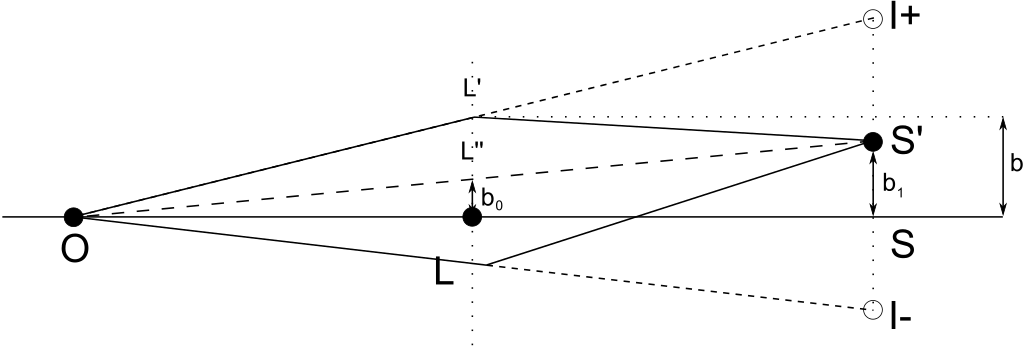
\includegraphics[width=0.9\textwidth]{Lens.jpeg}
\caption{Przykład zjawiska soczewkowania, gdzie źródło S' jest obserwowane jako dwa obrazy I+ i I- \citet{Lens}.}
\label{Fig1}
\end{figure}

\ak Obraz źródła widziany przez obserwatora może ulec różnym deformacjom, tj. rozciągnięciu, przemieszczeniu, kilkukrotnemu odbiciu, a także wzmocnieniu, co w przypadku tego projektu jest najistotniejszym aspektem soczewkowania. Przykłady takiego zjawiska przedstawiają Rysunki \ref{Fig2} i \ref{Fig3}.
\begin{figure}[H]
\begin{subfigure}{0.5\textwidth}
\centering
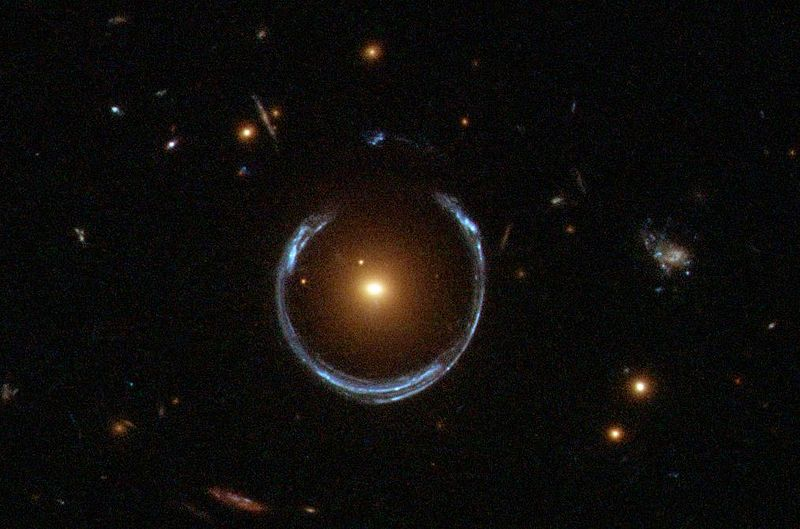
\includegraphics[width=0.9\linewidth,height=5cm]{Horseshoe.jpeg}
\caption{Galaktyka LRG 3-757 soczewkująca obraz galaktyki znajdującej się za nią \citet{Horseshoe}}
\label{Fig2}
\end{subfigure}
\hspace{0.5cm}
\begin{subfigure}{0.5\textwidth}
\centering
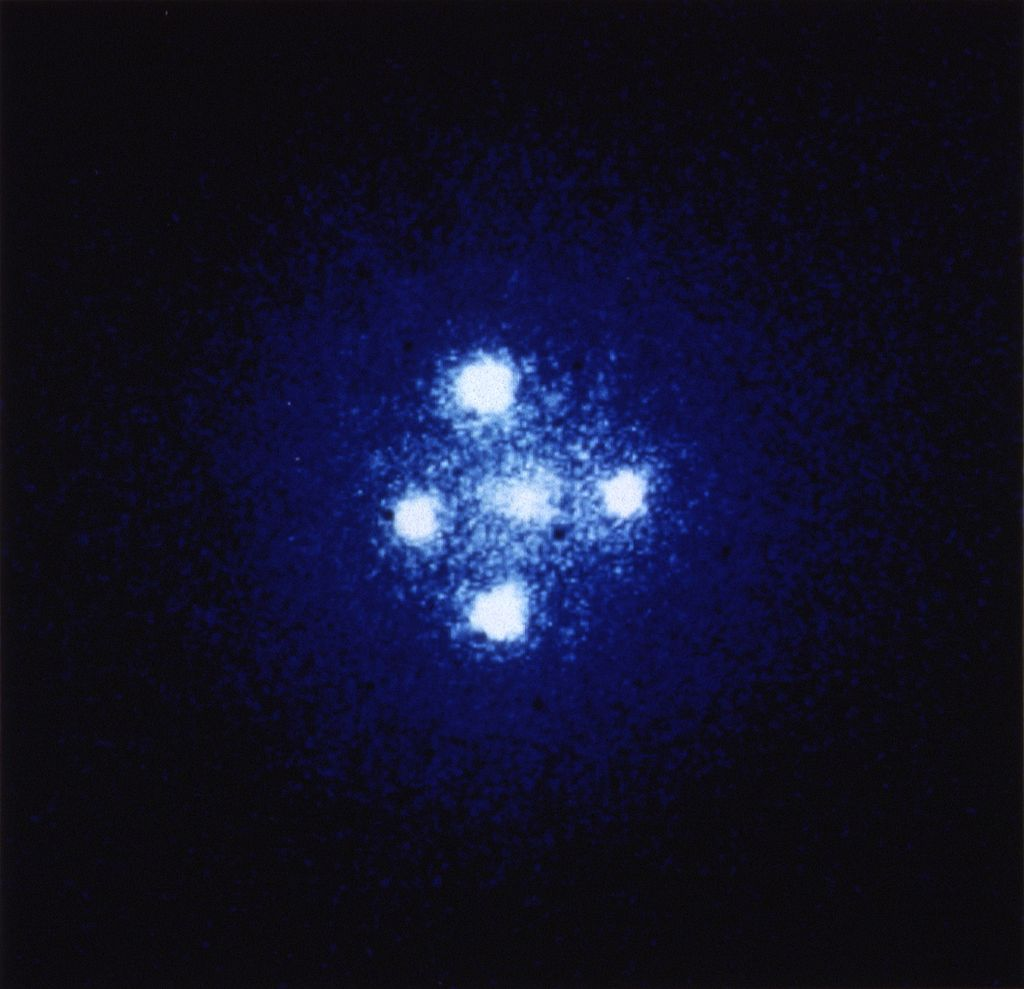
\includegraphics[width=0.9\linewidth,height=5cm]{Cross.jpeg}
\caption{Kwazar Q2237+030 soczewkowany przez galaktykę ZW 2237+030, tzw. krzyż Einsteina \citet{Cross}}
\label{Fig3}
\end{subfigure}
\caption{Przykłady deformacji obrazu spowodowane soczewkowaniem grawitacyjnym}
\end{figure}
\ak W szczególnych przypadkach, gdy masa soczewkująca jest stosunkowo nieduża, a jej tor ruchu przecina bądź jest bardzo bliski torowi promieni świetlnych od źródła do obserwatora, efekty deformacji obrazu mają zbyt małe rozmiary kątowe, by udało się je zaobserwować z Ziemi. W takich sytuacjach jedyną obserwowalną konsekwencją zajścia soczewki jest wzmocnienie jasności. Ten specyficzny rodzaj soczewkowania nazywany jest mikrosoczewkowaniem grawitacyjnym. Przykładem jego może być obiekt z pobliskiej galaktyki wysyłający ku Ziemi promieniowanie elektromagnetyczne, na którego drodze znajduje się masywna planeta. Wzmocnienie można wyrazić jako wielkość $\mu$, będącą ilorazem strumienia światła bez wzmocnienia oraz z wzmocnieniem. Ponieważ natężenie światła $I$ jest stałe w czasie, będzie to wyłącznie iloraz kątów bryłowych, z których światło dociera do  obserwatora.\\
\begin{equation}
\centering
\mu=\frac{Id\Omega}{Id\Omega_{0}}=\frac{d\Omega}{d\Omega_{0}}
\label{Eq_1}
\end{equation}
\flushleft
\ak Wzmocnienie można również dobrze opisać za pomocą odległości $u$ źródła światła od soczewki, którą można opisać za pomocą kilku parametrów, które dla danej soczewki można przyjąć jako stałe w trakcie trwania zjawiska. Wspomniane parametry geometryczne mają wpływ na $t_{E}$, tj. czas Einsteina. Wielkość $b$ jest wielkością analogiczną do parametru zderzenia i także jest stała. Czas $t_{0}$ jest momentem największego wzmocnienia, z kolei jedyną zmienną we wzorze \ref{Eq_2} jest czas {t}.
\begin{equation}
\centering
u(t)=\sqrt{\left(\frac{t-t_{0}}{t_{E}}\right)^{2}+b^{2}}
\label{Eq_2}
\end{equation}
\ak Znając już zależność $u(t)$ można powiązać ją ze wspomnianym wcześniej wzmocnieniem $\mu$, tj. wyprowadzić wzór \ref{Eq_3}, zwany także krzywą Paczyńskiego. Przykładową krzywą Paczyńskiego przedstawia Rysunek \ref{Fig_997}. %tutaj ref do krzywej w subsection "Projekt OGLE"
W skali sześciu lat mikrosoczewka trwająca ok. $70$ dni widocznie wyróżnia się skokiem jasności w trakcie trwania zjawiska, co było punktem wyjściowym przy konstrukcji algorytmu i zostanie opisane dokładniej w kolejnych rozdziałach.
\begin{equation}
\centering
\mu(u)=\frac{u^{2}+2}{u\sqrt{u^{2}+4}}
\label{Eq_3}
\end{equation}
\flushleft
\subsection{Projekt OGLE}

\ak Projekt OGLE  tj. ,,Optical Gravitational Lensing Experiment'' jest projektem naukowym prowadzonym w obserwatorium Las Campanas w Chile, przez Obserwatorium Astronomiczne Uniwersytetu Warszawskiego, w ramach którego m.in. wykonywane są pomiary jasności gwiazd, mające na celu poszukiwanie zjawisk mikrosoczewkowania. 

\ak Projekt kierowany jest przez prof. Andrzeja Udalskiego, a jego zasadniczym obszarem obserwacji są rejony w pobliżu centrum naszej galaktyki. Od początku istnienia projektu (kwiecień 1992 roku) zaobserwowano: 20 nowych planet pozasłonecznych, ponad 4000 zjawisk mikrosoczewkowania oraz kilkaset tysięcy nowych gwiazd zmiennych\footnote{Dane ze strony internetowej projektu: \textit{http://www.astrouw.edu.pl/index.php/ogle-artykul}}. Projekt jest aktualnie (od marca 2010 roku) w czwartej fazie realizacji. Poprzednie fazy miały miejsce w latach: 1992-1995 (OGLE-I), 1997-2001 (OGLE-II), 2001-2009 (OGLE-III) i wiązały się ze stosowaniem innych detektorów.
 

\section{Analiza danych}
\subsection{Dane}
\ak Dane na których oparty jest nasz projekt studencki pochodzą z projektu OGLE-III i zawierają 280.000 plików tekstowych w, którym znajduje się około 2400 pomiarów jasności w przeciągu 6 lat. Warto wspomnieć tutaj że jakość część pomiarów jest daleka do ideału i musieliśmy posegregować dane czy się nadają do analizy, np. w części plików były pojawiały się tylko jasności gwiazd 99,9 magnitudo co oczywiście nie sama sensu.
\subsection{Ogólnie o programie}
\ak Do analizy danych napiliśmy program w języku Python. Dokładny kod znajduje się na platformie github \url{https://github.com/wolf3213/Projekt-Astrolensing}. Składa się on z kilku części:
\begin{enumerate}
\item ,,Main'', czyli cześć główna programu
\item ,,Predictor'', czyli podprogram odpowiadający za ustalanie czy jest soczewka i obliczanie niepewnośći standardowej dla czasu $sigma_t$. Patrz: Opis algorytmu 2.4.
\item ,,Parser'', czyli podprogram czytający z pliku
\item ,,Curve'', czyli podprogram odpowiedzialny za przechowanie danych, tworzenie wykresów i wstępne odrzucanie szumów.
\end{enumerate} 
\subsection{Odsiew szumu}
\ak Właściwa część programu zaczynała się dopiero po wczytaniu danych. Wstępnie odfiltrowywał on wszystkie potencjalnie nienadające się do obróbki dane. Obejmowało to dane, które:
\begin{enumerate}
\item Zawierały pomiary jasności o wartości większej niż 99 magnitudo 
\item Zostały wykonane między 1. a 2137., oraz  2450. i 2500. dniem trwania projektu OGLE. Musieliśmy je usunąć, ponieważ nie nadawały się do analizy w związku z ilością błędów jakie one gerenowały.
\end{enumerate}

\subsection{Opis algorytmu}
\ak Program, operując już na nieodrzuconych danych, oblicza dla pomiarów jasności danej gwiazdy: odchylenie standardowe  $\sigma_{mag}$ i średnią $m_0$. Następnie  sprawdza, które pomiary jasności $m$ spełniają nierówność

\begin{equation}
m<\sigma_{mag}\cdot A+m_0 
\label{Eq_4}
\end{equation}
to znaczy są jaśniejsze niż średnia plus pewna wielokrotność $\sigma_{mag}$ i zlicza je, przy czym $A$ jest arbitralnie ustaloną dodatnią liczbą, wybraną przez programistę. Następnie dla punktów spełniających nierówność, liczy odchylenie standardowe po czasie $\sigma_t$, oraz średni czas $t$ tych punktów.\\
\ak Jeżeli teraz nasz plik z danymi zawiera n pomiarów spełniających nierówność (\ref{Eq_4})  i jeżeli $\sigma_t$ jest mniejsze niż $T$, to program zwraca nam informacje o podejrzeniu że w tym pliku może być soczewka, wraz z wykresem pomiarów jasności i naniesionym czasem $t$. Czas ten informuje nas kiedy, według programu zachodzi soczewkowanie.
\ak Zasadniczą ideą, którą się posługiwaliśmy jest fakt, że nasze soczewki będą jaśniejsze niż ,,większość'' pomiarów, przy czym dokładne znaczenie słowa ,,większość'' jest ustalone, przez wybór wartości $A$.
\\ 
\ak Drugim faktem, który dla nas jest kluczowy jest to informacja, że mikrosoczewki nie trwają dłużej niż 100-200 dni. A odchylenie standardowe czasu tj. $\sigma_t$ pozwoli nam określić rząd wielkości potencjalnej soczewki, co pozwoli nam odrzucić szumy.
\\
\subsection{Problemy}
Algorytm przedstawiony przez nasz zespół nie był pozbawiony mankamentów. Jego głównym celem było jak najsprawniejsze przesianie danych, które z pewnością nie są soczewkami. Głównymi problemami z którymi musimy się skonfrontować są: wstępne odrzucenie danych, które są soczewkami oraz konieczność ręcznego przejrzenia plików, które program zakwalifikował jako potencjalne soczewki. Przykładową krzywą blasku, którą program zakwalifikował jako soczewkę, a która w rzeczywistości jest gwiazdą zmienną przedstawia rysunek poniżej.
\begin{figure}[H]
\begin{subfigure}{0.5\textwidth}
\centering
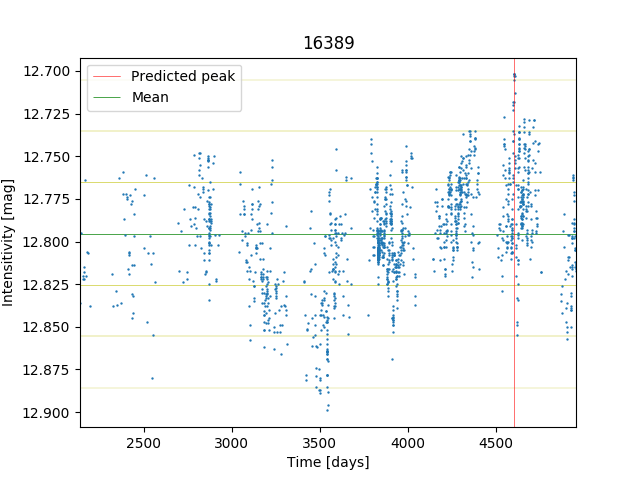
\includegraphics[width=\linewidth,height=5.5cm]{16389.png}
\label{Fig_10}
\end{subfigure}
\hspace{0.25cm}
\begin{subfigure}{0.5\textwidth}
\centering
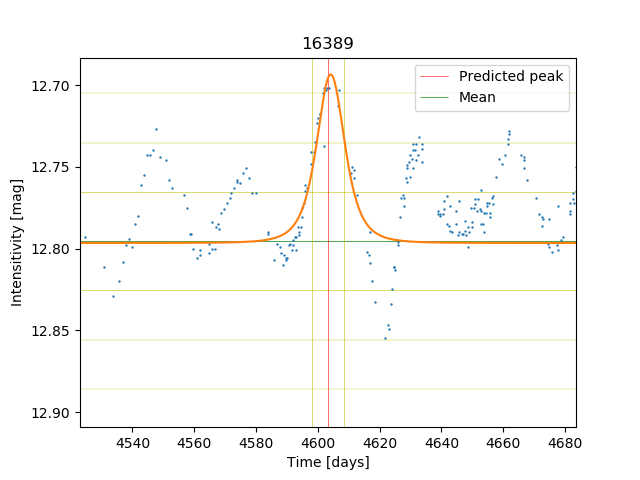
\includegraphics[width=\linewidth,height=5.5cm]{16389_v.png}
\label{Fig_11}
\end{subfigure}
\caption{Gwiazda zmienna w pliku 16389 zakwalifikowana przez algorytm jako soczewka}
\end{figure}
\section{Testy programu}
\ak W celu oszacowania jaki błąd pierwszego rodzaju jest generowany przez nasz program, wzięliśmy potwierdzone soczewki udostępnione na stronie OGLE, i sprawdziliśmy ile z nich zostanie wykryte przez program. Na program wykrywał 26 soczewek na 36 plików. Pliki na których przeprowadzone zostały testy zostały zapisane w folderze code/lens/ na naszym repozytorium na githubie.
\subsection{Znalezione soczewki}
\ak Uruchomiliśmy program na pełnych danych przy parametrach: 
$$A=3\textrm{, } T=30 \textrm{ i } n=5$$
\ak Według nas znaleźliśmy , przy tych parametrach 24 soczewki, 31 wykresów jasności jest do dalszej dyskusji, oraz przypadkowo 14 gwiazd zmiennych. Przykładowe wykresy jasności soczewek załączone są w podsekcji ,,Wizualizacje''. 
\begin{subsection}{Wizualizacje}
\ak Wynikiem działania programu są pliki graficzne w formacie .png, które przedstawiają dopasowaną krzywą Paczyńskiego do danych w momencie wystąpienia potencjalnej soczewki. Pliki zostały przez nas przejrzane i wybrane zostały z nich te, które wizualnie najbardziej odpowiadały faktycznemu wystąpieniu soczewki. Część z nich przedstawiliśmy na rysunkach poniżej.
\begin{figure}[H]
\begin{subfigure}{0.5\textwidth}
\centering
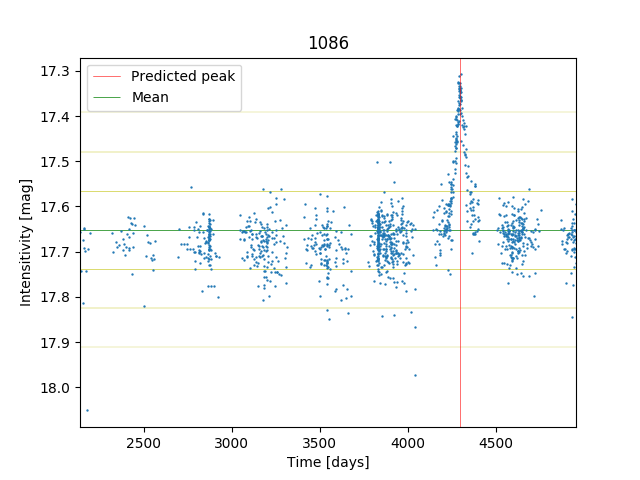
\includegraphics[width=\linewidth,height=5.5cm]{1086.png}
\label{Fig_4}
\end{subfigure}
\begin{subfigure}{0.5\textwidth}
\centering
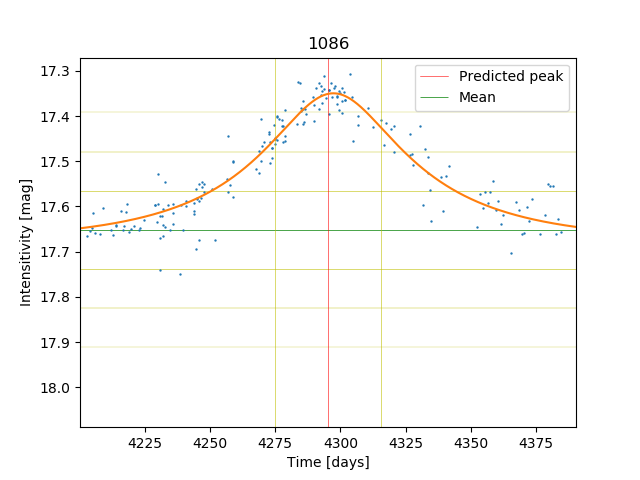
\includegraphics[width=\linewidth,height=5.25cm]{1086_v.png}
\label{Fig_5}
\end{subfigure}
\caption{Peak znaleziony wśród danych dla gwiazdy w pliku o numerze 1086 wraz z przybliżeniem i dopasowaną krzywą Paczyńskiego}
\end{figure}
\begin{figure}[H]
\begin{subfigure}{0.5\textwidth}
\centering
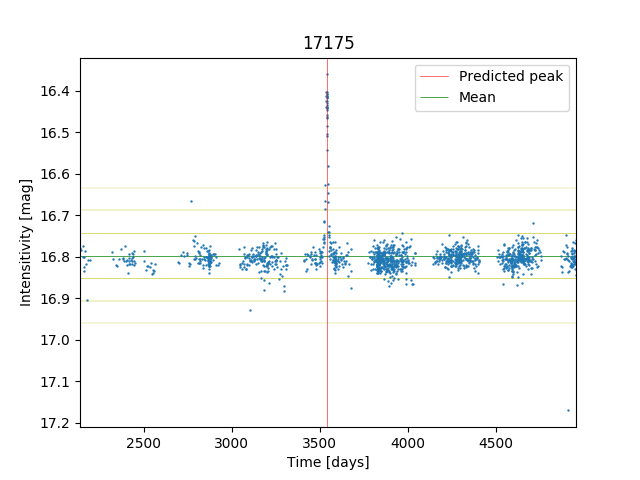
\includegraphics[width=\linewidth,height=5.25cm]{17175.png}
\label{Fig_6}
\end{subfigure}
\begin{subfigure}{0.5\textwidth}
\centering
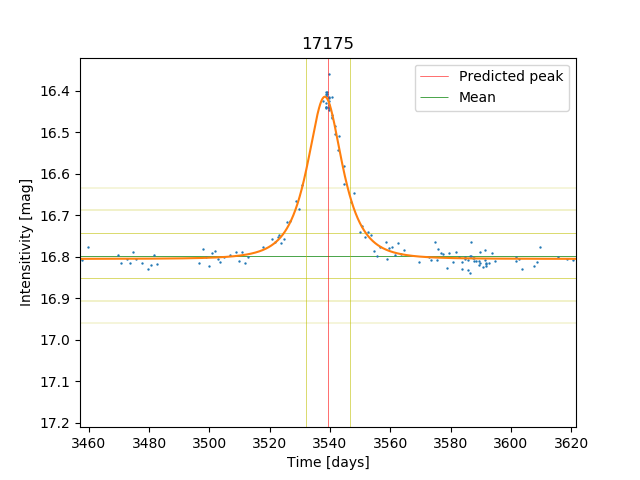
\includegraphics[width=\linewidth,height=5.25cm]{17175_v.png}
\label{Fig_7}
\end{subfigure}
\caption{Peak znaleziony wśród danych dla gwiazdy w pliku o numerze 17175 wraz z przybliżeniem i dopasowaną krzywą Paczyńskiego}
\end{figure}
\begin{figure}[H]
\begin{subfigure}{0.5\textwidth}
\centering
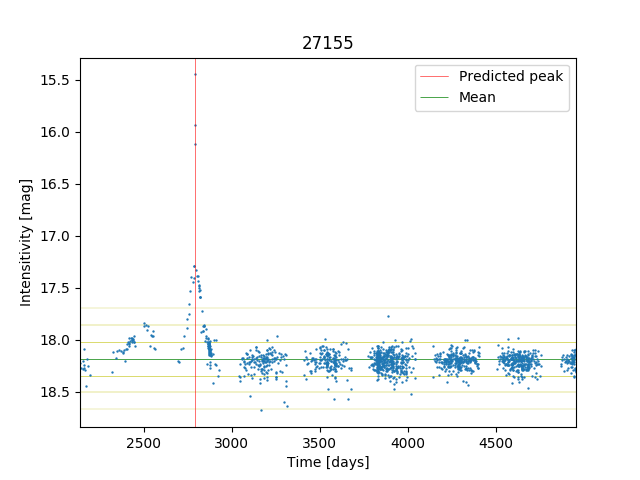
\includegraphics[width=\linewidth,height=5.25cm]{27155.png}
\label{Fig_8}
\end{subfigure}
\begin{subfigure}{0.5\textwidth}
\centering
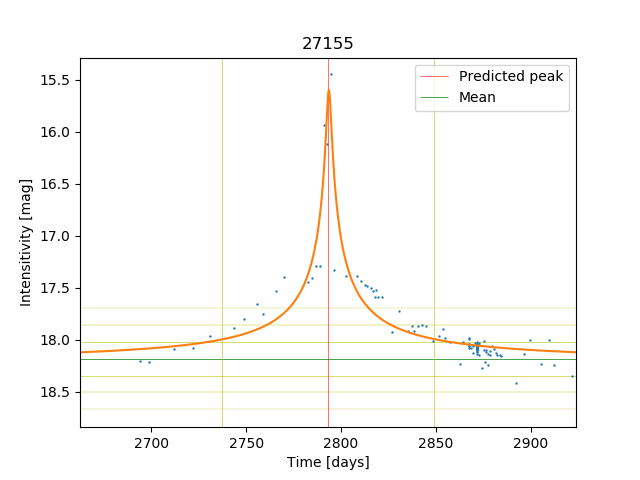
\includegraphics[width=\linewidth,height=5.25cm]{27155_v.png}
\label{Fig_9}
\end{subfigure}
\caption{Peak znaleziony wśród danych dla gwiazdy w pliku o numerze 27155 wraz z przybliżeniem i dopasowaną krzywą Paczyńskiego}
\end{figure}
\begin{figure}[H]
\begin{subfigure}{0.5\textwidth}
\centering
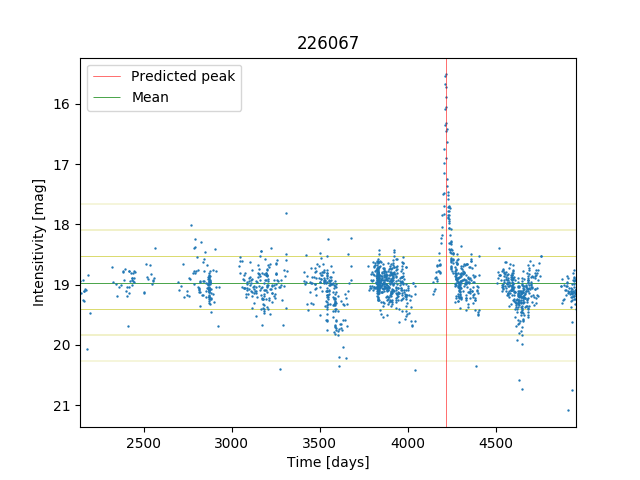
\includegraphics[width=\linewidth,height=5.25cm]{226067.png}
\label{Fig_12}
\end{subfigure}
\begin{subfigure}{0.5\textwidth}
\centering
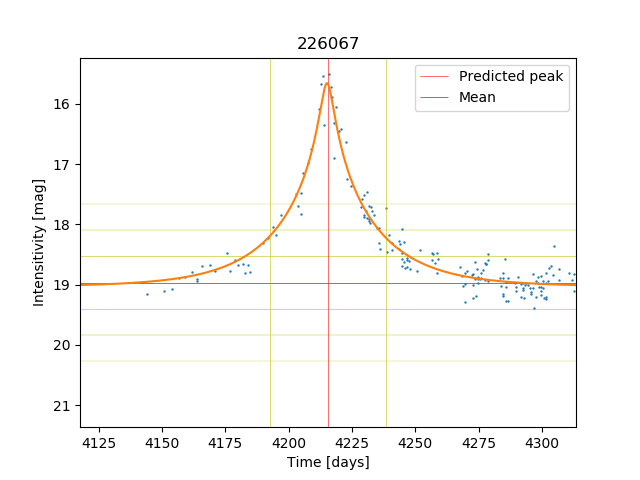
\includegraphics[width=\linewidth,height=5.25cm]{226067_v.png}
\label{Fig_13}
\end{subfigure}
\caption{Peak znaleziony wśród danych dla gwiazdy w pliku o numerze 226067 wraz z przybliżeniem i dopasowaną krzywą Paczyńskiego}
\end{figure}
\end{subsection}
\bibliography{bibliografia}
\end{document}